\subsection{Page Packing After 4~KiB Compression}\label{sec:binpacking}

\begin{figure}
    \centering
    \begin{subfigure}[b]{0.3\linewidth}
        \centering
        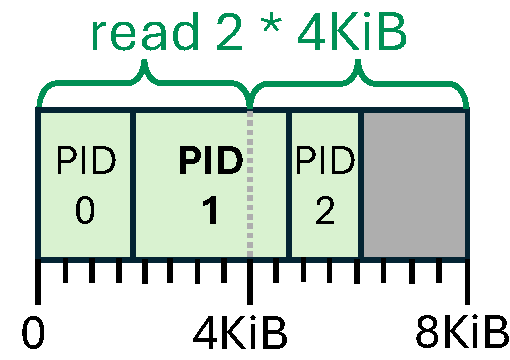
\includegraphics[width=0.95\linewidth]{figures/binpacking0.pdf}
        \caption{Read with \\ 4~KiB granularity}
        \label{fig:binpacking0}
    \end{subfigure}
    \hfill
    \begin{subfigure}[b]{0.3\linewidth}
        \centering
        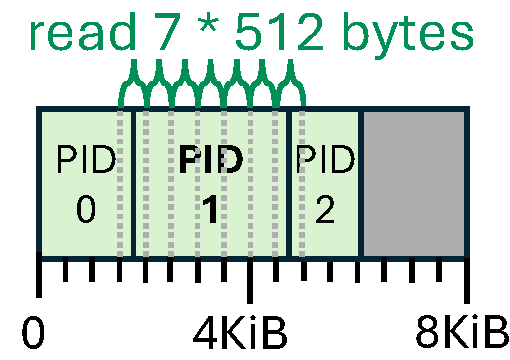
\includegraphics[width=0.95\linewidth]{figures/binpacking1.pdf}
        \caption{Read with \\ 512~B granularity}
        \label{fig:binpacking1}
    \end{subfigure}
    \hfill
    \begin{subfigure}[b]{0.3\linewidth}
        \centering
        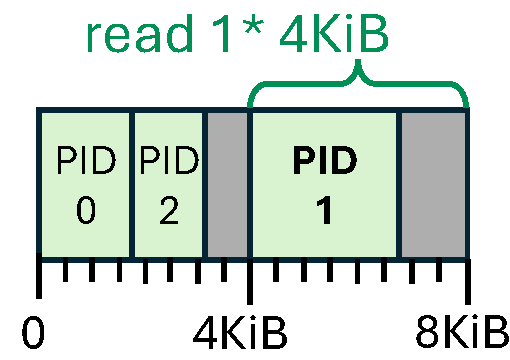
\includegraphics[width=0.95\linewidth]{figures/binpacking2.pdf}
        \caption{Read PID stored \\ by page packing}
        \label{fig:binpacking2}
    \end{subfigure}
    \caption{Total amount of reads when reading PID 1}
    \label{fig:binpacking}
    \vspace{-3mm} 
\end{figure}

\module{Read is optimal with 4~KiB granularity and alignment.}  
Read latency strongly influences transaction latency~\cite{DBLP:journals/pacmmod/NguyenAZL25}. 
To identify the optimal read unit, we run an FIO microbenchmark~\cite{fio} on four enterprise SSDs: random reads from 512~B to 8~KiB in 512~B steps, aligned to request size. % ; for two FDP‑enabled SSDs (A, B) that, in our setup, exposed only 4~KiB reads, we used 4~KiB and 8~KiB.
Each test ran for 30~minutes, with a single thread for latency (QD=1), and 32 threads (QD=64) for throughput.
Across all models, aligned 4~KiB requests achieved the lowest latency and highest throughput:
\begin{center}
  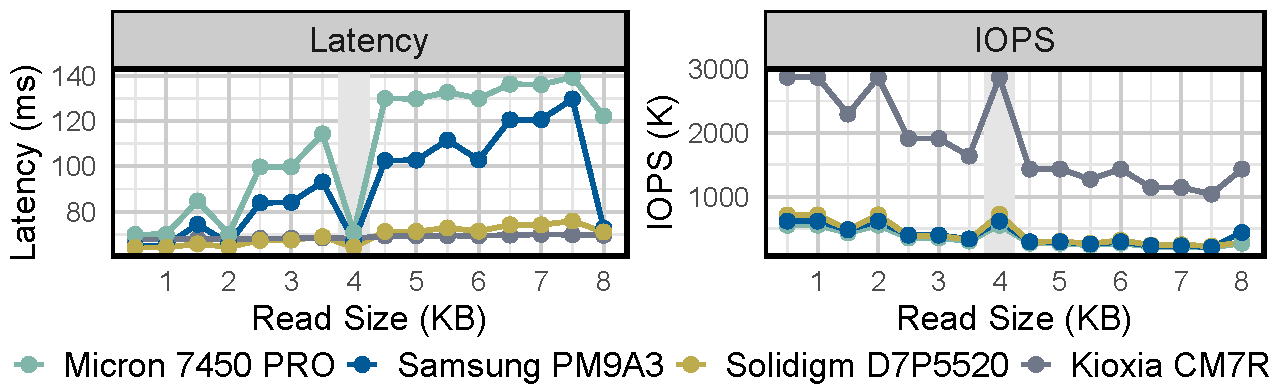
\includegraphics[clip, width=0.88\columnwidth]{figures/read.pdf}
\end{center}
\noindent
Smaller or misaligned requests, in contrast, incur additional internal reads~\cite{DBLP:journals/pvldb/HaasL23}.
Hence, 4~KiB is the most efficient size and alignment granularity for reading compressed pages.  


% \begin{figure}
%     \centering
%     \begin{subfigure}[b]{0.49\linewidth}
%         \centering
%         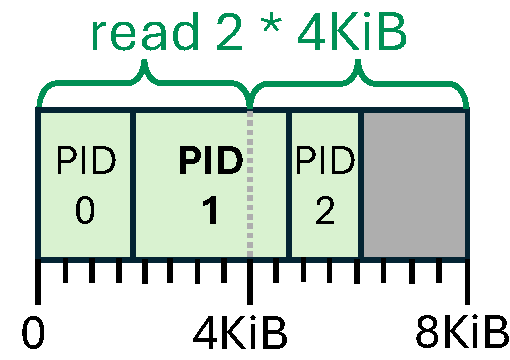
\includegraphics[width=0.64\linewidth]{figures/binpacking0.pdf}
%         \caption{Reading an unaligned page with 4~KiB granularity}
%         \label{fig:binpacking0}
%     \end{subfigure}
%     \hfill
%     \begin{subfigure}[b]{0.49\linewidth}
%         \centering
%         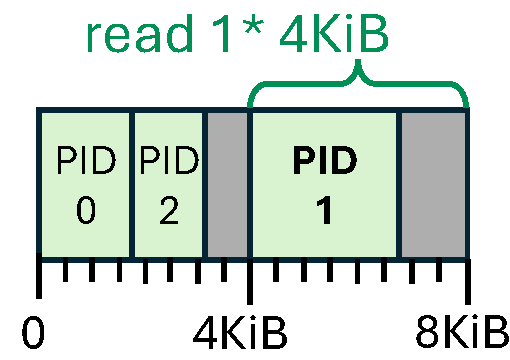
\includegraphics[width=0.64\linewidth]{figures/binpacking2.pdf}
%         \caption{Reading a page stored by\\page packing}
%         \label{fig:binpacking2}
%     \end{subfigure}
%     \caption{Total amount of reads when reading PID 1}
%     \label{fig:binpacking}
% \end{figure}


\module{Read amplification can occur depending on the placement.}
Using 4~KiB pages with per-page compression yields variable-sized pages that, if poorly placed, can become misaligned on disk.
Such misalignment negates compression benefits by preserving write and space costs while introducing read amplification: a single PID read may trigger multiple physical reads~\cite{DBLP:journals/pvldb/HaasL23}.
For example, a 3{,}000~byte compressed page that crosses a 4~KiB boundary requires two 4~KiB reads, totaling $\approx2.73\times$ its size (\cref{fig:binpacking0}).
Even with 512~B reads, it still incurs $\approx1.19\times$ amplification (\cref{fig:binpacking1}).
This increases read latency and eliminates the intended compression gains.

\module{Optimization: 4~KiB-aligned page packing.}
To ensure each compressed page is retrievable with a single 4~KiB read, we use \emph{page packing}: align each compressed page to a 4~KiB boundary.
When writing a batch (e.g., 64 pages), we compress each page and place it into 4~KiB slots via a best‑fit binpacking algorithm~\cite{DBLP:journals/jal/Baker85}. 
Compressed pages never cross 4~KiB boundaries (\cref{fig:binpacking2}).
Compared to unaligned 4~KiB or 512~B reads, page packing lets each PID be fetched with one 4~KiB access---cutting I/Os relative to unaligned 4~KiB reads and remaining faster than 512‑byte reads.
In short, 4~KiB page packing yields fast, predictable reads with minimal amplification (with a small amount of bounded internal slack per page).

\begin{figure}
  \centering
  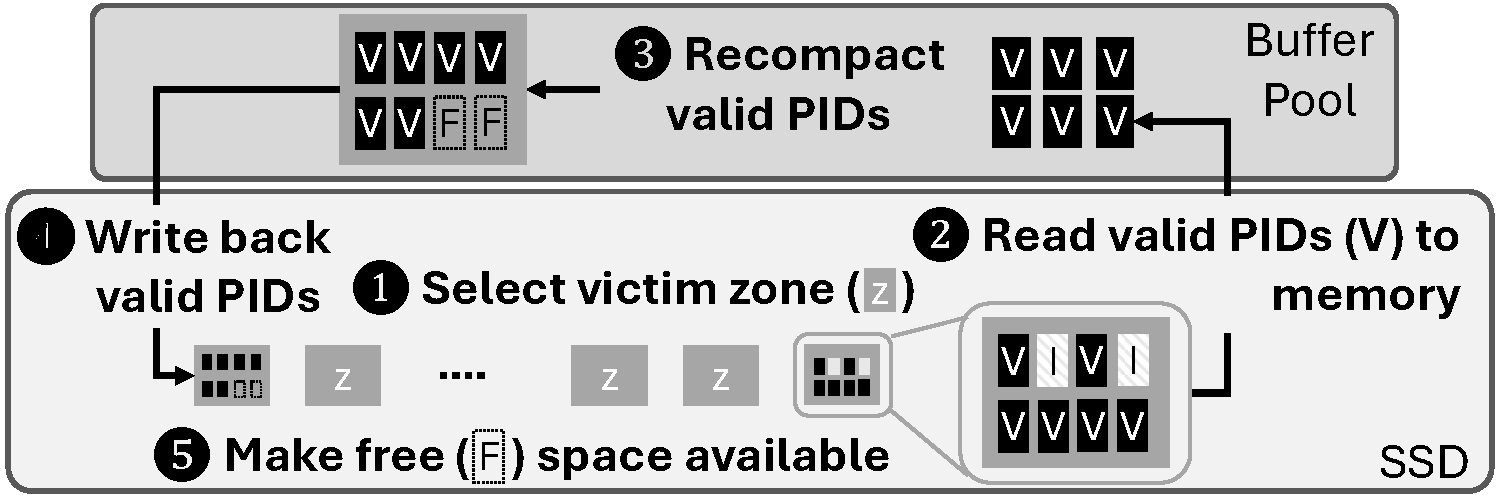
\includegraphics[clip, width=0.8\columnwidth]{figures/GC.pdf}
  \caption{Garbage collection process}
  \label{fig:gc}
\end{figure}
